\section{8080-Interface mittels SRAM-Interface}
\label{sec:TeilA_8080SRAM}
Wie bereits in \refc{cha:gnublin_extended} erwaehnt, besitzt der Prozessor des Gnublin bereits ein externes 8080-Interface, auf welches zugegriffen wird. Im Folgenden wird auf das Konzept, die Idee und die Realisierung auf Hardware- und Softwareseite eingegangen.
\newpage
\subsection{Konzept}
Im Gnublin stellt ein NXP LPC313x die zentrale Recheneinheit dar. Dieser besitzt ein sogenanntes EBI \footnote{EBI: External Bus Interface}, worüber externe Bausteine wie Speicher, Ethernetcontroller oder ähnliche Bausteine angesprochen werden können. 


\begin{figure}[htp]
%\begin{minipage}[t]{0.8\textwidth}
%\begin{figure}[h]
	\centering
	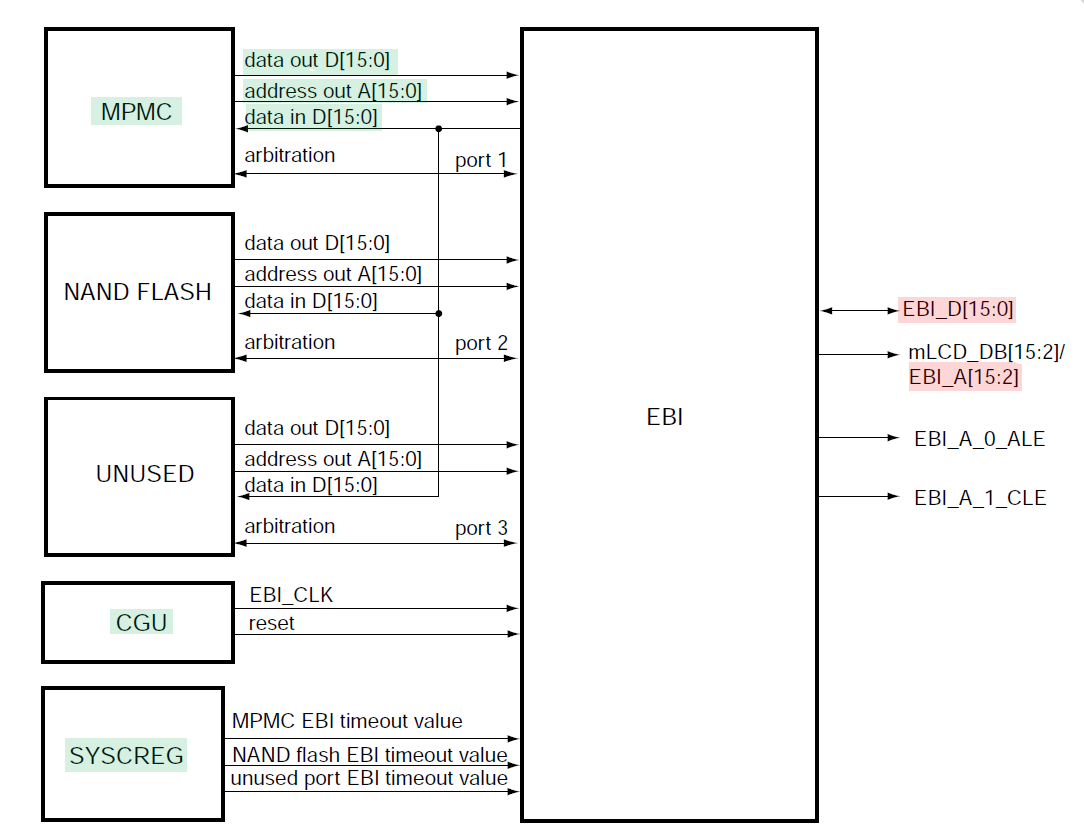
\includegraphics[width=1.0\textwidth]{TeilA/lpc_ebi.png}
	\caption{NXP LPC313x EBI, Quelle: \cite{NXP2010}}
	\label{fig:lpc_ebi}
\end{figure}
%\end{minipage}

In \refa{fig:lpc_ebi} ist ein Blockschaltbild des EBI zu sehen, bei welchem neben CGU \footnote{CGU: Clock Generation Unit, Takterzeugung} und SYSCREG\footnote{SYSCREG: System Control Register, Steuerregister}, MPMC\footnote{MPMC: Multiport Memory Controller} sowie das NAND Flash an den Eingängen des EBI angeschlossen sind. An den Ausgängen des EBI sind Adress- und Datenbus zum Anschluss an externe Bausteine herausgeführt. Damit verschiedenartigen Bausteine an denselben Adress- und Datenpins angeschlossen werden kann, ist eine Priorisierung notwendig. Die Höchste Priorität besitzt der MPMC, gefolgt vom NAND Flash. 
Die Grundidee ist, das Display über den MPMC anzuschließen, da er so konfiguriert werden kann, dass er sich 8080-konform verhält.


\subsection{MPMC - Multiport Memory Controller des NXP LPC313x}

Der MPMC stellt die Möglichkeit zur Verfügung Bausteine wie dynamisches und statisches RAM anzubinden. Die Refresh-Zyklen werden bei Verwendung von dynamischen RAMs automatisch vollzogen. Das SDRAM-Interface bietet von Haus aus die Möglichkeit Displays mit 8080-Interface zu betreiben. Dies schließt allerdings die Verwendung von dynamischen RAMs aus. Soll ein Betriebssystem wie Linux laufen, ist allerdings die Verwendung von dynamischem RAM unerlässlich. Im Folgenden wird die Schnittstelle für das statische RAM SRAM-Interface benannt. Es besteht die Möglichkeit das Interface des statischen RAM zu verwenden, um ein Display zu betreiben, da es sich so konfigurieren lässt, dass es sich wie ein 8080-Interface verhält. Damit sich die verschiedenen Slaves an Adress- und Datenbus nicht überschneiden, regelt das EBI den Zugriff auf die Busse über Chip-Select Leitungen. Am Gnublin ist eine dieser Chip-Select-Leitungen fuer das SRAM-Interface nach außen gelegt. Die restlichen Anschlüsse wie Write-Enable, Read-Enable sind ebenfalls herausgeführt \cite{NXP2010}.


\begin{figure}[tbph]
%\begin{figure}[h!]
	\centering
	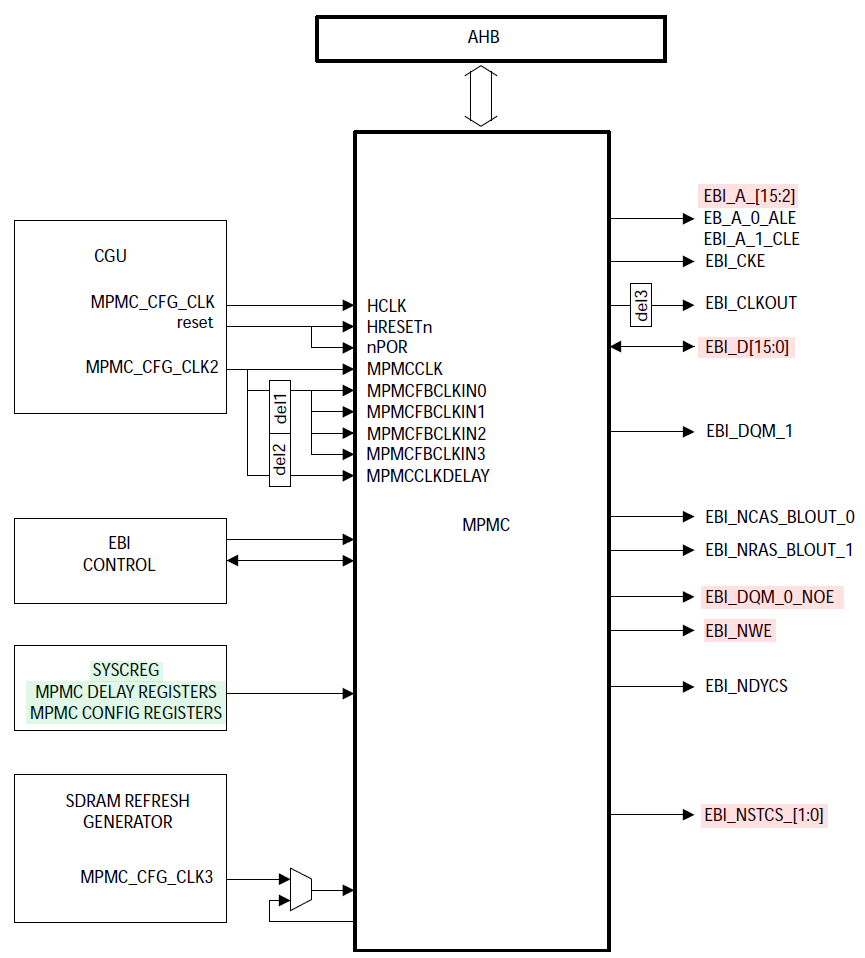
\includegraphics[width=1.0\textwidth]{TeilA/lpc_mpmc.png}
	\caption{NXP LPC313x MPMC, Quelle: }
	\label{fig:lpc_mpmc}
\end{figure}
\newpage
Die Register des MPMC werden so konfiguriert, dass die Schnittstelle kompatibel zum Display und dessen Timings wird. Entsprechend dem verwendeten Chip-Select-Signal werden die Register MPMCStaticConfig0, MPMCStaticWaitWen0, MPMCStaticWaitOen0, MPMCStaticRd0, MPMCStaticPage0, MPMCStaticWr0 und MPMCStaticWaitTurn0 entsprechend \reft{tab:mpmc_config} konfiguriert. Die Basisadresse des MPMC ist 0x1700 8000.

\begin{table}[h]
\begin{tabular}{|p{4cm}|p{1cm}|p{1cm}|p{6.6cm}|}\hline
%\begin{tabular}{|c|c|c|c|}\hline
	\textbf{Register} 	& \textbf{Offset} 	& \textbf{Wert} & \textbf{Beschreibung} 							\\ \hline
	MPMCStaticConfig0 	& 0x200 		& 0x81 			& 16 Bit Modus, Aktiviert die Nutzung von EBI\_nWE 	\\ \hline
	MPMCStaticWaitWen0 	& 0x204 		& 13 			& 13 + 1 = 14 Wartezyklen ab Chi- Select bis Write-Enable 	\\ \hline
	MPMCStaticWaitOen0 	& 0x208 		& 0 			& 0 + 1 = 1 Wartezyklus ab Chip-Select bis Output-Enable  												\\ \hline
	MPMCStaticRd0 		& 0x20C 		& 0 			& 0 + 1 = 1 Wartezyklus ab Chip-Select bis Read-Enable					\\ \hline
	MPMCStaticPage0 	& 0x210 		& 0 			& 0 + 1 = 1 Wartezyklus für sequential Page Mode Access												\\ \hline
	MPMCStaticWr0 		& 0x214 		& 15 			& 15 + 2  = 17 Wartezyklen bis Write-Access	\\ \hline
	MPMCStaticWaitTurn0 & 0x218 		& 0 			& 0 + 1 = 1 Turnaround Cycles 								\\ \hline
\end{tabular}
\caption{MPMC Register}
\label{tab:mpmc_config}
\end{table}


\subsection{Hardwareverbindung zwischen SRAM-Interface und Display (Adapterplatine)}

\subsection{Software}
\subsubsection{Entwicklung eines Linux-Framebuffer-Treibers}
\paragraph{Anpassungen für Display mit SSD1289 Controller}
\paragraph{Anpassungen für Display mit SSD1963 Controller}
\paragraph{Anpassungen für Display mit CPLD Controller}
\subsubsection{Entwicklung eines User-Space-Treibers}
\paragraph{Anpassungen für Display mit SSD1289 Controller}
\paragraph{Anpassungen für Display mit SSD1963 Controller}
\paragraph{Anpassungen für Display mit CPLD Controller}
\subsubsection{Anpassung des APEX-Bootloaders zur Verwendung des Displays}
\subsubsection{Probleme bei der Entwicklung und Fehlersuche}
\paragraph{Probleme mit SSD1963}
\subparagraph{Rolle des User-Space-Treibers}
\subparagraph{Debuggen mit Logik-Analyzer}



